\documentclass[10pt,oneside,a4paper]{article}
\usepackage[utf8]{inputenc}
\usepackage{amsmath}
\usepackage{indentfirst}
\usepackage{enumitem}
\usepackage[spanish]{babel}
\usepackage[export]{adjustbox}
\usepackage{graphicx}
\graphicspath{ {img/} }
\usepackage{listings}
\usepackage{subfig}
\usepackage{cite}
\usepackage{pgfplots}

\addtolength{\oddsidemargin}{-.300in}
\addtolength{\evensidemargin}{-.300in}
\addtolength{\textwidth}{0.600in}
\addtolength{\topmargin}{-.300in}
\addtolength{\textheight}{0.600in} %1.75

\begin{document}
\begin{titlepage}

\title{\Huge Procesadores Gráficos y Aplicaciones en Tiempo Real  \\[0.7in] \LARGE Sistema de partículas por GPU\\[3.6in]}
\date{}
\author{Álvaro Muñoz Fernández\\
Iván Velasco González}
\maketitle
\thispagestyle{empty}
\end{titlepage}

\section{Introducción}
El objetivo de esta práctica consiste en la implementación de un modelo de partículas básico implementado en shaders de cómputo que se ejecutarán en GPU. Además se proponen tareas adicionales, de las que se ha optado por la implementación de la ordenación de partículas (también realizada en shaders de cómputo) para una correcta visualización de las partículas.

\section{Aplicación cliente}
La aplicación se ha implementado en C++ partiendo de un proyecto vacío en el que se han añadido las librerías necesarias para el desarrollo. Se ha utilizado \textit{freeGLUT} para la inicialización del contexto, \textit{GLEW} para la inicialización de extensiones, \textit{GLM} para las funciones matemáticas y estructuras de datos algebraicas, y \textit{FreeImage} para la carga de texturas, aunque finalmente no se ha cargado ninguna textura en el proyecto.\\

El proyecto se divide en funciones de inicialización, funciones de cómputo y funciones de renderizado que son llamadas en los puntos de ejecución donde son necesarias. Además se emplean estructuras de datos para almacenar la información correspondiente a los programas utilizados.

\section{Sistema de partículas}
El sistema de partículas que se ha implementado es el propuesto por Mike Bailey, que incluye solamente colisiones entre las partículas y una esfera definida mediante su posición y radio. Opcionalmente podía extenderse este sistema, pero nosotros hemos optado por la implementación de ordenación y renderizado con transparencia.\\

\begin{figure}[h!tbp]
\centering
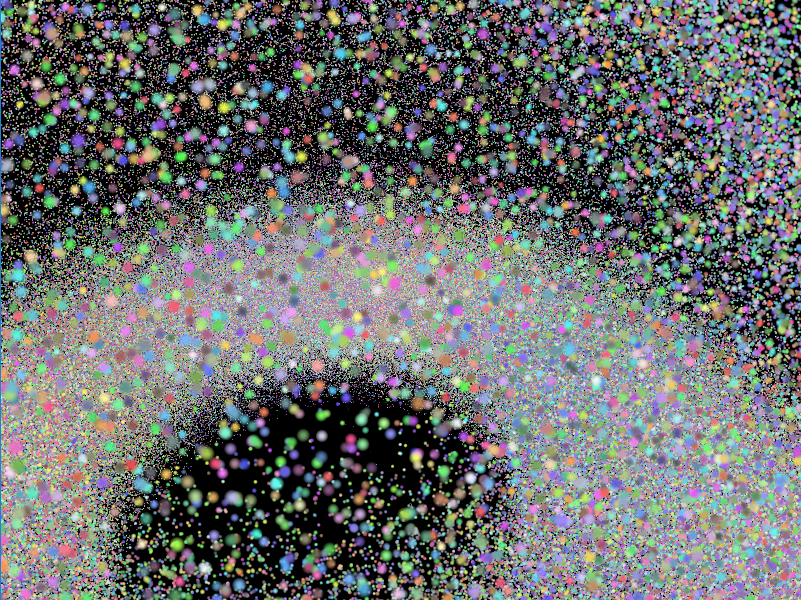
\includegraphics[width=.8\linewidth]{img/particles.png}
\caption{Instantánea del sistema de partículas}
\end{figure}

El sistema de partículas se almacena en tres buffers que contienen las posiciones, velocidades y colores de las partículas.

\section{Ordenación}
\subsection{Inicialización}
Antes de proceder a la ordenación de las partículas es necesario inicializar dos buffers extra. Uno de ellos almacena los índices que se emplearán en la llamada \textit{DrawElements()} para realizar el dibujado ordenado, y el otro almacenará las distancias de cada partícula a la cámara.\\

Este paso previo se realiza en una shader de cómputo que exclusivamente almacena, de forma paralela, la distancia de cada una de las partículas en el array de distancias.

\subsection{Ordenación}
La ordenación se realiza en una nueva shader de cómputo que realiza varias pasadas. Hemos optado por una implementación de \textit{bitonic sort}, que recibe el buffer de distancias y el buffer de índices y realiza la ordenación solamente del buffer de índices.\\

Con este buffer ordenado puede realizarse el renderizado ordenado a través de un VAO sin necesidad de modificar los buffers con información de partículas. Se ha tomado esta decisión porque aunque incrementa el uso de memoria, simplifica el número de accesos ya que se escribe sobre un solo buffer de valores enteros utilizando la información leída de un buffer auxiliar, en lugar de modificar los 3 buffers de información de cada partícula, cada uno de ellos con 3 elementos float por cada partícula.

\section{Renderizado}
\subsection{Billboards}
\begin{figure}[h!tbp]
\centering
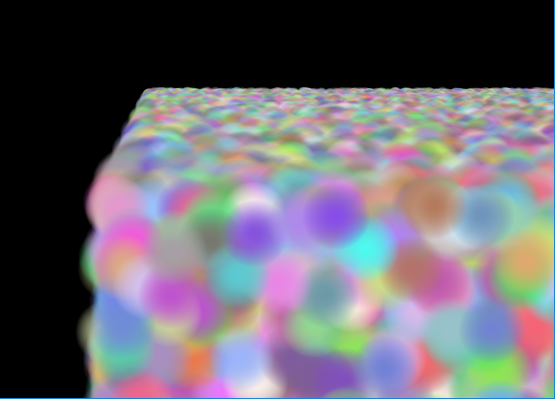
\includegraphics[width=.8\linewidth]{img/billboards.png}
\caption{Varios billboards orientados a cámara}
\end{figure}
Para dibujar cada una de las partículas se ha creado una shader de geometría que recibe las posiciones de las partículas como puntos y las traslada a posiciones en el espacio de cámara. En este espacio el eje Y está orientado perpendicularmente a la cámara, por lo que al generarse un quad siempre estará orientado hacia la cámara. De esta forma se consigue el efecto billboard con facilidad, generándose los quads sobre los que dibujar la partícula de forma eficiente en la shader de geometría. Además se generan coordenadas UV en cada vértice de la partícula que permitirán colorear correctamente la partícula en la shader de fragmentos.

\subsection{Texturizado}

\begin{figure}[h!tbp]
\centering
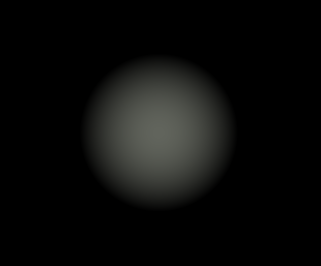
\includegraphics[width=.8\linewidth]{img/proceduraltexture.png}
\caption{Visualización de una partícula con transparencia}
\end{figure}
Para colorear las partículas se utiliza el color que se asigna aleatoriamente al inicio de la simulación. En lugar de utilizar una textura como máscara, se ha generado procedimentalmente la máscara de las partículas. Mediante la distancia al centro de la partícula se calcula el porcentaje de opacidad de la partícula, decayendo este cuanto más lejos del centro está un fragmento. Así se consigue una forma esférica suavizada para las partículas, con una transparencia variable que permite que algunas zonas sean translúcidas y se vea con facilidad el resultado de la aplicación del blending.

\section{Funcionamiento de la demo}
\subsection{Tamaño de partícula}
Se ha añadido funcionalidad para alterar el tamaño de partícula en tiempo de ejecución. Esto puede hacerse mediante las teclas \textbf{+} y \textbf{-}.

\subsection{Pausa de simulación}
La simulación se puede pausar y reanudar presionando la tecla \textbf{P}.

\subsection{Reinicio de simulación}
La simulación se puede reiniciar presionando la tecla \textbf{R}.

\subsection{Alternar ordenado}
El ordenado de partículas puede activarse y desactivarse presionando la tecla \textbf{T}.

\subsection{Estadísticas}
Presionando la tecla \textbf{L} se muestran por consola las estadísticas de la media de frametime y framerate de los últimos 50 frames.

\subsection{Cámara}
La cámara se puede manipular mediante las teclas \textbf{W}, \textbf{A}, \textbf{S}, \textbf{D} y con el movimiento del ratón mientras se mantiene presionado el botón izquierdo. Además se puede alterar la elevación de la cámara utilizando la tecla \textbf{Espacio} para ascender y \textbf{Z} para descender.

\section{Análisis de resultados}
\subsection{Media de resultados por ejecución}
\centering {
\begin{tikzpicture}
\begin{axis}[
	x tick label style={
		/pgf/number format/1000 sep=},
	ylabel=Frametime(ms),
	enlargelimits=0.05,
	legend style={at={(0.5,-0.1)},
	anchor=north,legend columns=-1},
	ybar interval=0.7,
]
\addplot
	coordinates {(16,8.225863) (128,8.225863)
	 (512,8.225863)};
\addplot
	coordinates {(16,8.225863) (128,8.225863)
	 (512,8.225863)};
\addplot
	coordinates {(16,8.225863) (128,8.225863)
	 (512,8.225863)};
\addplot
	coordinates {(16,8.225863) (128,8.225863)
	 (512,8.225863)};
\legend{Total,Físicas,Ordenación,Render}
\end{axis}
\end{tikzpicture}
}

\end{document}